\section{Experimental validation}
\label{sec:exp}

\subsection{Setup and design}

The entire campaign runs inside a public continuous-integration workflow on a
standard hosted runner with four virtual cores, 16~GB of memory and no
persistent state; nothing outside a personal account and a container runtime is
required, and every result is reproducible by re-running the workflow. Each job
provisions a Hyperledger Besu~\cite{besu} QBFT network of $\n$ validators from a
generated genesis, each validator confined to a control group with CPU
quota~$\q$ and a fixed memory limit as required by Definition~\ref{def:rnm}.
A closed-loop generator drives $\cc$ concurrent workers issuing value-transfer
transactions and measures committed throughput over a steady-state interval
after a warm-up, discarding runs whose coefficient of variation across the final
third exceeds a preset tolerance.

Faults are injected at the network level with kernel traffic control on the
validator interfaces, producing packet loss and duplication on the peer-to-peer
links of the designated subset; since the transport is encrypted this realizes
the omission class of Definition~\ref{def:faults} but not equivocation, and the
paper claims nothing about the latter. The detector polls the client's signer
metrics to obtain per-validator participation counts over a window of $\w$
rounds, so that $\pd$, $\pf$, $\rho$ and the receiver-operating characteristic
are estimated from observed behaviour rather than assumed, and the sweep over
the threshold~$\thr$ yields the Youden operating point used in
Section~\ref{sec:case}.

The design comprises six measured groups and four post-hoc analyses.
\textbf{X1} sweeps $\n\in\{4,5,7,9,11,13,16\}$ at fixed $\cc=16$ to estimate
$\beta$ under the \RNM{} protocol; \textbf{X2} repeats a coarser $n$-grid at
three quota levels to test $\q$-invariance (Statement~\ref{st:qinvariance});
\textbf{X3} sweeps $\cc\in\{1,2,4,8,16,32,64\}$ at $\n=7$ to estimate $\gamma$,
$\csat$ and $\theta$, the union of the reference-quota X1 $n$-sweep with the
unsaturated part of X3 forming the calibration set for the joint
fit~\eqref{eq:ols}; \textbf{X4} adds emulated wide-area round-trip times to
obtain $\beta(\mathrm{RTT})$; \textbf{X5} injects omission and duplication over
a grid of loss rates with faulty fraction $\phi=0.2$ to characterize the
detector; and \textbf{X9} was specified as a cross-client replication on a
second QBFT-family implementation but did not yield usable throughput records
in this campaign, so all calibrated coefficients below are Besu-only. The
remaining analyses require no new runs: \textbf{X3b} re-samples the calibration
data along artificial concurrency paths $\lambda\in\{0,0.5,1,2\}$ to test the
identifiability theorem, \textbf{X6} extrapolates by discrete-event simulation,
\textbf{X7} assesses predictive coverage on the held-out counts
$\resHoldoutN$, and \textbf{X8} is the sizing ablation. The whole campaign
comprises $\resTotalRuns$ successful measurement records and about
$\resCoreHours$ core-hours, with the largest directly measured validator set
$\resNmaxMeasured$.

\subsection{Results}

The joint fit~\eqref{eq:ols} on the reference-quota calibration subset
(unsaturated $c$-sweep together with the $n$-sweep at its design concurrency)
gives
$\beta=\resBeta\pm\resBetaSE$ and $\gamma=\resGamma\pm\resGammaSE$ with
coefficient of determination $\resRsq$ in log-space; the remaining calibrated
parameters and their standard errors are collected in the upper block of
Table~\ref{tab:results}. The sign of $\beta$ is the first substantive check:
under the \RNM{} protocol one must have $\beta>0$ (throughput declines with
$\n$), as replicated state machine semantics require, whereas a single-factor
fit on the same measurements re-sampled along $\lambda=1$ yields
$\ahat=\resAlphaHat$ against the predicted $\gamma\lambda-\beta=\resAlphaPred$.

\begin{figure}[!t]
\centering
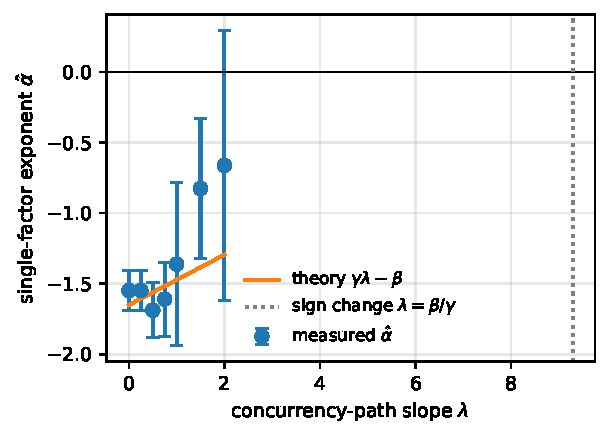
\includegraphics[width=0.75\textwidth]{figures/fig_confounding}
\caption{Experiment~X3b. Single-factor exponent $\ahat$ estimated from data
re-sampled along concurrency paths of slope~$\lambda$, against the prediction
$\gamma\lambda-\beta$ of Theorem~\ref{thm:identifiability}. The predicted sign
change is at $\lambda=\beta/\gamma=\resLambda$}
\label{fig:confounding}
\end{figure}

Figure~\ref{fig:confounding} shows the sweep: estimated exponents track the
predicted line $\gamma\lambda-\beta$. With the calibrated ratio
$\beta/\gamma=\resLambda$ the sign change lies above the concurrency paths
realized in the load-generator design, so every measured single-factor exponent
in the campaign remains negative --- yet the $\lambda=1$ point already
reproduces the classical confound of Theorem~\ref{thm:identifiability} to within
sampling error. The middle block of Table~\ref{tab:results} reports the
accompanying invariance tests: the partial $F$-test for
quota\,$\times\log\n$ interaction has $p=\resQinvP$, so exact $\q$-invariance
is rejected on the full X2 grid and the bi-factor coefficients above are
therefore reported at the reference quota $\q=0.25$ only; $\beta$ estimated
under zero and elevated round-trip time moves from $\resBetaRttZero$ to
$\resBetaRttHigh$.

\begin{table}[!t]
\centering
\caption{Calibrated parameters, invariance and detector characteristics, and
predictive coverage}
\label{tab:results}
\begin{tabular}{lll}
\headline
Quantity & Estimate & Note \\
\headline
$\Tzero$ & $\resTzero$ & normalized scale \\
$\beta$ & $\resBeta\pm\resBetaSE$ & consensus exponent \\
$\gamma$ & $\resGamma\pm\resGammaSE$ & concurrency exponent \\
$\csat$, $\theta$ & $\resCsat$, $\resTheta$ & saturation \\
$\hat\sigma$ & $\resSigmaRes$ & log-residual s.d. \\
\hline
$\ahat$ at $\lambda=0,\,1,\,2$ & $\resAlphaHatL0$, $\resAlphaHatL1$, $\resAlphaHatL2$
 & \textit{cf.}\ $\gamma\lambda-\beta$ \\
$\beta$ by quota $0.20,0.25,0.33$ & $\resBetaQlow$, $\resBetaQmid$, $\resBetaQhigh$
 & X2 \\
$q$-invariance $F$-test & $p=\resQinvP$ & Statement~\ref{st:qinvariance} \\
$\beta$ at RTT $0$, high & $\resBetaRttZero$, $\resBetaRttHigh$ & X4 \\
$\pd$, $\pf$, $\rho$ & $\resPd$, $\resPf$, $\resRho$ & at $\thr=\resDetectorThr$ \\
detector AUC & $\resAuc$ & X5 \\
\hline
held-out $\n$ & $\resHoldoutN$ & coverage set \\
coverage at $90\%$ & $\resCovNinety$ & nominal $0.90$ \\
coverage at $95\%$ & $\resCovNinetyFive$ & nominal $0.95$ \\
\headline
\end{tabular}
\end{table}

The lower block reports predictive coverage on the held-out validator counts,
which is the check that decides whether the intervals of Statement~\ref{st:pi}
may be used for sizing. An out-of-sample comparison of four predictors --- a
linear model, a single-factor power law, the Universal Scalability
Law~\cite{gunther2007} and~\eqref{eq:bifactor} --- gives held-out log-space
RMSE $\resRmseLinear$, $\resRmseSingle$, $\resRmseUsl$ and $\resRmseOurs$
respectively. The sizing ablation of Section~\ref{sec:case} further reports
relative provisioning cost under the same four predictors as
$\resCostLinear$, $\resCostSingle$, $\resCostUsl$ and $\resCostOurs$.
